%  article.tex (Version 3.3, released 19 January 2008)
%  Article to demonstrate format for SPIE Proceedings
%  Special instructions are included in this file after the
%  symbol %>>>>
%  Numerous commands are commented out, but included to show how
%  to effect various options, e.g., to print page numbers, etc.
%  This LaTeX source file is composed for LaTeX2e.

%  The following commands have been added in the SPIE class 
%  file (spie.cls) and will not be understood in other classes:
%  \supit{}, \authorinfo{}, \skiplinehalf, \keywords{}
%  The bibliography style file is called spiebib.bst, 
%  which replaces the standard style unstr.bst.  

\documentclass[]{spie}  %>>> use for US letter paper
%%\documentclass[a4paper]{spie}  %>>> use this instead for A4 paper
%%\documentclass[nocompress]{spie}  %>>> to avoid compression of citations
%% \addtolength{\voffset}{9mm}   %>>> moves text field down
%% \renewcommand{\baselinestretch}{1.65}   %>>> 1.65 for double spacing, 1.25 for 1.5 spacing 
%  The following command loads a graphics package to include images 
%  in the document. It may be necessary to specify a DVI driver option,
%  e.g., [dvips], but that may be inappropriate for some LaTeX 
%  installations. 
\usepackage[]{graphicx}

\usepackage{subfig}
\usepackage{verbatim}
\usepackage{amsmath}
\usepackage{amssymb}
\usepackage{algpseudocode}
\usepackage{algorithm}

\newcommand{\stdfigure}[3]{ \begin{figure}[htp] \centering \includegraphics[width=0.95\linewidth]{#1} \caption{#3} \label{fig:#2} \end{figure} }
\newcommand{\stdfigurevar}[4]{ \begin{figure}[htp] \centering \includegraphics[width=#4\linewidth]{#1} \caption{#3} \label{fig:#2} \end{figure} }
\newcommand{\stdfigurefull}[3]{ \begin{figure*}[htp] \centering \includegraphics[width=0.95\linewidth]{#1} \caption{#3} \label{fig:#2} \end{figure*} }
\newcommand{\stdfigurefullvar}[4]{ \begin{figure*}[htp] \centering \includegraphics[width=#4\linewidth]{#1} \caption{#3} \label{fig:#2} \end{figure*} }

\newcommand{\fig}[1]{Figure~\ref{fig:#1}}
\newcommand{\figf}[1]{Figure~\ref{fig:#1}}
\newcommand{\figsub}[2]{Figure~\ref{fig:#1}\,(#2)}
\newcommand{\figsubf}[2]{Figure~\ref{fig:#1}\,(#2)}
\newcommand{\figsubref}[2]{Figure~\ref{fig:#1}\,\subref{fig:#2}}
\newcommand{\figsubreff}[2]{Figure~\ref{fig:#1}\,\subref{fig:#2}}
% not figure how to remove () from subref
\newcommand{\figsubrefrange}[3]{Figure~\ref{fig:#1}\,\subref{fig:#2}-\subref{fig:#3}}
\newcommand{\figsubrefrangef}[3]{Figure~\ref{fig:#1}\,\subref{fig:#2}-\subref{fig:#3}}

\newcommand{\eq}[1]{Eq.~(\ref{eq:#1})}
\newcommand{\eqf}[1]{Equation~(\ref{eq:#1})}

\newcommand{\sect}[1]{Section~\ref{sec:#1}}
\newcommand{\sectf}[1]{Section~\ref{sec:#1}}

\newcommand{\tbl}[1]{Table~\ref{tbl:#1}}
\newcommand{\tblf}[1]{Table~\ref{tbl:#1}}

\newcommand{\dataset}[1]{Dataset~#1}
\newcommand{\datasetf}[1]{Dataset~#1}

\newcommand{\alg}[1]{Algorithm~\ref{alg:#1}}
\newcommand{\algf}[1]{Algorithm~\ref{alg:#1}}
% \newcommand{\algl}[2]{Algorithm~\ref{alg:#1} line #2}
% \newcommand{\alglf}[2]{Algorithm~\ref{alg:#1} line #2}
% \newcommand{\algls}[2]{Algorithm~\ref{alg:#1} lines #2}
% \newcommand{\alglsf}[2]{Algorithm~\ref{alg:#1} lines #2}
\newcommand{\lne}[1]{line~\ref{ln:#1}}
% \newcommand{\lns}[1]{lines #1}
% \newcommand{\lnf}[1]{Line #1}
% \newcommand{\lnsf}[1]{Lines #1}

\newcommand{\red}[1]{\textcolor{red}{#1}}
\newcommand{\yellow}[1]{\textcolor{red}{#1}}
\newcommand{\green}[1]{\textcolor{green}{#1}}

\newcommand{\rem}[1]{\pdfmarkupcomment[markup=StrikeOut,color=red,author=JW]{#1}{removed}}
% \newcommand{\add}[1]{\pdfmarkupcomment[markup=Highlight,author=JW,color=yellow,opacity=1.0]{#1}{added}}
\newcommand{\add}[1]{\yellow{#1}}
% \newcommand{\upd}[1]{\pdfmarkupcomment[markup=Highlight,author=JW,color=green,opacity=1.0]{#1}{to update}}
\newcommand{\upd}[1]{\green{#1}}
\newcommand{\com}[2]{\pdfmarkupcomment[markup=Highlight,author=JW,color=blue,opacity=1.0]{#1}{#2}}

\newcommand{\ncite}[1]{}
\newcommand{\ncaption}[1]{}

\newcommand{\prop}[1]{Property~(#1)}
\def\props{properties}
\def\fprops{Properties}

\def\data{unary}
\def\smooth{binary}
\def\dataf{Unary}
\def\smoothf{Binary}

\def\obj{substructure}

\def\pslice{U_k}
\def\nslice{U_{k+1}}

\def\eg{e.g.}
\def\etal{et al.}
\def\etc{etc.}
\def\ie{i.e.}

\title{Interactive Grain Image Segmentation using Graph Cut Algorithms} 

%>>>> The author is responsible for formatting the 
%  author list and their institutions.  Use  \skiplinehalf 
%  to separate author list from addresses and between each address.
%  The correspondence between each author and his/her address
%  can be indicated with a superscript in italics, 
%  which is easily obtained with \supit{}.

\author{Jarrell Waggoner\supit{a}, Youjie Zhou\supit{a}, Jeff Simmons\supit{b}, Ayman Salem\supit{b}, \\ Marc De Graef\supit{c}, and Song Wang\supit{a}
\skiplinehalf
\supit{a}University of South Carolina, Columbia, SC 29208, USA; \\
\supit{b}Materials and Manufacturing Directorate, Air Force Research
Labs, Dayton, OH 45433, USA; \\
\supit{c} Carnegie Mellon University, Department of Materials Science and Engineering, 5000 Forbes Avenue, Pittsburgh, PA, 15213, USA
}

%>>>> Further information about the authors, other than their 
%  institution and addresses, should be included as a footnote, 
%  which is facilitated by the \authorinfo{} command.

\authorinfo{Further author information: (Send correspondence to J. Waggoner)\\
J. Waggoner: E-mail: waggonej@email.sc.edu, Telephone: 847-261-4747\\ 
Y. Zhou: E-mail: zhou42@email.sc.edu \\ 
J. Simmons: E-mail: jeff.simmons@wpafb.af.mil \\ 
A. Salem: E-mail: ayman.salem.ctr@wpafb.af.mil \\ 
M. De Graef: E-mail: degraef@cmu.edu \\
S. Wang: E-mail: songwang@cec.sc.edu, Telephone: 803-777-2487}
%%>>>> when using amstex, you need to use @@ instead of @


%%%%%%%%%%%%%%%%%%%%%%%%%%%%%%%%%%%%%%%%%%%%%%%%%%%%%%%%%%%%% 
%>>>> uncomment following for page numbers
% \pagestyle{plain}    
%>>>> uncomment following to start page numbering at 301 
%\setcounter{page}{301} 
 
  \begin{document} 
  \maketitle 

%%%%%%%%%%%%%%%%%%%%%%%%%%%%%%%%%%%%%%%%%%%%%%%%%%%%%%%%%%%%% 
\begin{abstract}
% \input{spie-abstract.tex}
Segmenting materials images is a laborious and time-consuming process
and automatic image segmentation algorithms usually contain
imperfections and errors.  Interactive segmentation is a growing topic
in the areas of image processing and computer vision, which seeks to
find a balance between fully automatic methods and fully-manual
segmentation processes. By allowing minimal and simplistic interaction
from the user in an otherwise automatic algorithm, interactive
segmentation is able to simultaneously reduce the time taken to
segment an image while achieving better segmentation results. Given
the specialized structure of materials images and level of
segmentation quality required, we show an interactive segmentation
framework for materials images that has two key contributions: 1) a
multi-labeling framework that can handle a large number of structures
while still quickly and conveniently allowing manual interaction in
real-time, and 2) a parameter estimation approach that prevents the
user from having to manually specify parameters, increasing the
simplicity of the interaction.  We show a full formulation of each of
these contributions and example results from their application.
\end{abstract}

%>>>> Include a list of keywords after the abstract 

\keywords{image segmentation, materials volume segmentation,
  segmentation propagation, interactive segmentation, graph-cut
  approaches}

%%%%%%%%%%%%%%%%%%%%%%%%%%%%%%%%%%%%%%%%%%%%%%%%%%%%%%%%%%%%%

\section{Introduction}
\label{sec:intro}

Interactive segmentation is a rapidly-growing area of computer vision
and has seen heightened interest recently\cite{kuang:12,straehle:12}.
While traditional segmentation seeks to identify objects/structures
within an image in a fully-automated fashion, interactive
segmentation, similar to active learning~\cite{settles:09},
accomplishes the goal of image segmentation while incorporating a
sparse number of user interactions which are included as additional
constraints or guideance in the segmentation model or algorithm.
These interactions may take on different forms, and may include
drawing a bounding box~\cite{rother:04}, roughly outlining a
boundary~\cite{mortensen:95}, or drawing brush strokes inside and/or
outside the object of interest~\cite{santner:10, unger:08, boykov:01b,
  vezhnevets:95}.  A desired property of an interactive segmentation
approach is that the user interaction be as convenient (\ie, low
cognitive load) and sparse (\ie, few in number) as possible, while
simultaneously providing immediate feedback to the user on every
interaction.

Many existing methods segment the object of interest using a model
learned from user interactions~\cite{boykov:01b, unger:08, rother:04}.
Other approaches incorporate interaction into morphological operations
(watershed)~\cite{straehle:12}, co-segmentation~\cite{batra:10}, or
incorporate machine-learning to aid in the interactive
process~\cite{top:11, kuang:12}.  These interactive methods have been
applied to a number of domains, including natural
images~\cite{rother:04}, medical images~\cite{boykov:00}, and
neuroimages~\cite{straehle:11, straehle:12}.

One domain that has been unaddressed in interactive segmentation
literature is materials science image segmentation, where there are no
existing techniques focusing solely on segmenting materials images
using an interactive approach.  Materials science is especially
important to the development of new metals and biomaterials, and
presents unique challenges in image segmentation.  First, materials
images often are 3D volumes~\cite{ibrahim:91} made up of a sequence of
individual 2D image ``slices,'' as shown by the two sample slices in
\fig{full-ex}.  This large number of slices must all be segmented to
fully and properly analyze the 3D structure of the material.  Second,
depending on the inter-slice distance, the 2D structure in two
neighboring slices may show high continuity.  Such inter-slice
structure continuity must be considered to achieve accurate
segmentation.  Third, materials volumes consist of numerous
substructures (\eg,``grains'' in a metallic material, or ``cells'' in
a biomaterial, etc.) with complex relationships (\eg,
adjacency/nonadjacency relationships) among them that determine many
desirable properties of the material~\cite{swiler:95, rollett:04}.
Existing interactive segmentation techniques often only focus on
foreground-background segmentation~\cite{rother:04, boykov:01b}, and
may not scale to the large number of substructures present in
materials images.  Other methods may handle multiple
structures~\cite{straehle:11, straehle:12}, but do not incorporate any
prior knowledge about the unique relationships among substructures in
materials images~\cite{reed:06, tan:04}.  Finally, the imaging
techniques used to obtain a materials image volume may result in
significant noise or other ambiguities that increases the difficulty
to segment a materials image volume in a fully-automatic fashion.

There are a number of existing, non-interactive approaches to segment
materials images~\cite{chuang:08, simmons:09}.  Among the most
prominent is the work of Comer~\etal~\cite{comer:94, comer:00} on the
EM/MPM algorithm, originating from~\cite{marroquin:87}.  Other methods
that have been specifically used on materials images include graph
cut~\cite{landis:11, waggoner:11}, stabilized inverse diffusion
equations~\cite{huffman:08}, Bayesian methods~\cite{comer:11,
  simmons:08}, and the watershed~\cite{liq:07} method.  Most often,
materials images are opportunistically segmented by the simplest tools
available, such as thresholding~\cite{gonzalez:08,shapiro:01}, or
out-of-the-box methods such as watershed or normalized cut.  However,
these methods do not incorporate any interaction for manual refinement
by a user.  Since some of these approaches may require significant
time to run, requiring the user to examine and correct problems only
after the algorithm is complete may not be practical if rapid
refinement is desired.  Conversely, the general-purpose interactive
segmentation techniques discussed previously do not incorporate any
specific domain knowledge about materials images, and thus may require
additional effort on the part of the user than may otherwise be needed
when segmenting a materials image volume.

In this paper, we present an interactive segmentation approach to
segment materials science image volumes.  We show that an existing
propagation-based materials image segmentation
approach~\cite{waggoner:11} can be extended to allow for convenient
interactive segmentation.  We illustrate the performance of the
proposed approach by using it to segment a materials image volume
using smaller number of interactions compared with general-purpose
interactive segmentation methods that do not incorporate
materials-specific priors.  Finally, we develop methods to estimate
the parameters of this proposed approach to further reduce the number
of user-required interactions in the segmentation process.

The remainder of this paper is organized as follows: in
\sect{interactive} we discuss the proposed interactive segmentation
approach for materials image volumes. In \sect{param}, we show how
some of the parameters of the proposed method can be automatically
estimated.  In \sect{ex}, we evaluate the proposed method's
performance against another general-purpose interactive segmentation
method.  Finally, in \sect{conclusion} we provide brief concluding
remarks.

\section{Interactive Materials Image Segmentation}
\label{sec:interactive}

In~\cite{waggoner:11} we developed a 3D materials science image
segmentation method by propagating segmentation $S^U$ of a slice $U$
to a neighboring slice $V$, resulting in a segmentation $S^V$.  This
way, using an initial segmentation on one slice, we can repeatedly
propagate this segmentation to the remaining slices in the volume to
obtain a complete 3D segmentation.  This propagation was done while
preserving the topology (\ie, non-adjacency relations among 2D
segments), which led to a better performance when compared with
methods that did not incorporate topology as a prior.  %% More formally,
%% we define propagation as the process of transferring a known
%% segmentation to the remaining unsegmented slices.
\begin{figure}[htbp]
\centering
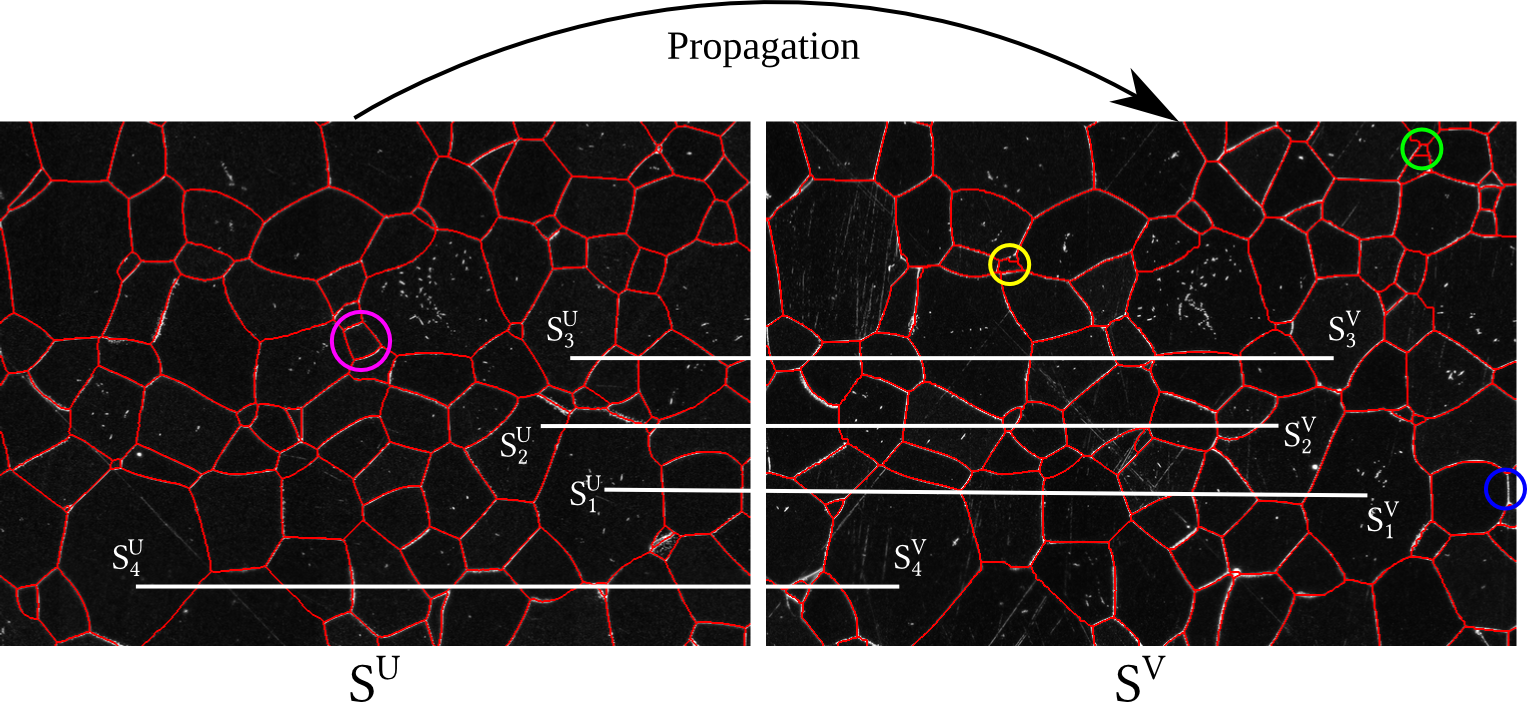
\includegraphics[width=\linewidth]{fig/dd}
\caption{Example of segmentation propagation, highlighting different
  types of topology changes.  Further discussion in the
  text.} \label{fig:full-ex}
\end{figure}
Specifically, let the segmentation
\[S^U = \{ S^U_1, S^U_2, \ldots, S^U_n \} , \]
where $S^U_i , i=1\ldots n$ are disjoint segments in slice $U$, and
this collection of segments makes up a partition of the slice $U$,
\[ U = \bigcup_{i=1}^{n} S^U_i . \] 
An example is shown in \fig{full-ex} where all the segments (``grain''
structures) are separated by red lines.  To propagate segmentation
$S^U$ to a new slice $V$ to yield the segmentation $S^V$, we minimize
the energy
\begin{equation}
  E( S^V ) = \sum_{p\in V}\Theta_p(S^V_i) + 
  \sum_{\{p,q\}\in\mathcal{P}^V_n} \Phi_{pq}(S_i^V , S_j^V)
\label{eq:energy1}
\end{equation}
where $\mathcal{P}^V_n$ is the set of all 4-connected pixels.  The
\data{} term $\Theta_p(S^V_i)$, which represents a cost for a pixel
$p$ being assigned to a segment $S^V_i$ in slice $V$, was set to
reflect the structure continuity between $U$ and
$V$,
\begin{equation}
  \Theta_p(S^{V}_i) = \left\{
    \begin{array}{lcr}
      0, &  \textrm{distance}(p,S^U_i) < d  \\
      \infty, & \textrm{ otherwise} \\
    \end{array}
  \right.
  \label{eq:theta}
\end{equation}
where $d$ is a dilation distance that reflects the maximum possible
structural change between $U$ and $V$~\cite{waggoner:11}.  In
addition, the \smooth{} term $\Phi_{pq}(S_i^V , S_j^V)$, which
represents a cost for a pair of neighboring pixels $p,q$ being
assigned to two (possibly the same) segments $S^V_i, S^V_j$, was
constrained to preserve \emph{non-adjacency} segment relationships
from $U$ to $V$; \ie, any two segments $S^V_i, S^V_j$ are allowed to
be adjacent (have pixels that are 4-connected between them) if the
corresponding segments in $S^U_i, S^U_j$ are also adjacent,
\begin{equation} \Phi_{pq}(S^V_i , S^V_j) = \left\{
    \begin{array}{lcr}
      0, & i = j \\
      \infty, & \{ S^U_i, S^U_j \} \notin \mathcal{A}^U  \\
      g( p, q ), & \{ S^U_i, S^U_j \} \in \mathcal{A}^U \\
    \end{array}
  \right. ,
  \label{eq:phi}
\end{equation}
where $\mathcal{A}^U$ contains segment pairs that are adjacent in
$S^U$, and we set $g(p,q)$ to reflect the image boundary information
in $V$~\cite{waggoner:11}.  An example is shown in \fig{full-ex},
where $S^V_1$ and $S^V_2$ are allowed to be adjacent because $S^U_1$
and $S^U_2$ were adjacent in $S^U$.  However, $S^V_1$ and $S^V_4$ have
an infinity penalty because $S^U_1$ and $S^U_4$ are not adjacent in
$S^U$.  This topology constraint was found to be particularly
important for materials images, and our proposed method was able to
outperform other methods that did not incorporate such a prior.

While finding the global minimum to this cost is NP-hard, this cost
has been shown to be minimizable to a local optimum using a graph-cut
approach~\cite{veksler:99, boykov:01}.  However, one phenomenon that
was observed in this previous work was that, during propagation, 2D
structure topology between $U$ and $V$ might not always be fully
consistent.  For example, a new 3D structure with no intersection in
slice $U$ might appear in slice $V$, \eg, the structure in the yellow
circle in \fig{full-ex}.  Similarly, a 3D structure intersected by
slice $U$ might disappear in slice $V$, such as the structure circled
in magenta in \fig{full-ex}.  This breaks the topology constraints
given in \eq{phi} in some local regions.  This may lead to spurious
segments and missing structures, as circled in green and blue
respectively, in \fig{full-ex}.  

The previous method made use of a brute-force automated search to
locate such spurious and missing structures in $V$~\cite{waggoner:11}.
However, particularly when the inter-slice distance is too large, it
is not possible to examine every location for possible spurious or
missing structures.  In this paper, our goal is to develop effective
interactive tools to allow a user to conveniently specify the local
areas that contain spurious or missing structures, and incorporate
such interactions to refine the segmentation $S^V$ to a corrected
$\tilde{S}^V$ on slice $V$, using the same energy minimization
algorithm.  more specifically, we propose to allow the user to correct
these two types of segmentation errors within this framework by: a)
annotating the location of a new segment to handle cases where a new
structure appears in slice $V$, and b) annotation of existing segments
that should no longer be present in segmentation $S^V$.

These interactions are inherently local because the 2D cross section
of a 3D structure shows very small size before appearing or
disappearing from a neighboring 2D slice.  Therefore, correcting $S^V$
to $\tilde{S}^V$ can be achieved by using the same energy
minimization in a local image areas around the interactive
annotations.  This is also important because interactive segmentation
requires instantaneous user feedback.  The previous propagation method
segmented entire slices, which was more computationally intensive than
is desirable in an interactive system.  We will further discuss these
two interactions, and how we identify local regions for each, in the
following subsections.

\subsection{Removal of Spurious Segments}
\label{sec:remove}

For this interaction, we allow the user to select a spurious segment
$S^V_k$ for removal by clicking the mouse on this segment in a
visualized segmentation of $S^V$.  Instead of naively removing this
segment by arbitrarily merging it into one of its neighbors, we use
the same energy minimization discussed above to assign the individual
pixels in $S^V_k$ to potentially different neighboring segments.  As
discussed above, we identify a local region in which we update the
segmentation.  Specifically, this local region consists of the
specified $S^V_k$ and its neighboring segments, \eg, $S^V_1, S^V_2,
S^V_3$ surrounding the spurious segment $S^V_k$ in
\figsub{removal-ex}{a}, and re-run the energy minimization within this
local region after modifying the $\Theta$ term to incorporate the
interaction, resulting in an updated segmentation in this local
region, as shown by the example in \figsub{removal-ex}{b}.
\begin{figure}[htbp]
\centering
\subfloat[]{
\includegraphics[width=0.32\linewidth]{fig/aaa.pdf}}
\hspace{0.1em}
\subfloat[]{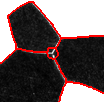
\includegraphics[width=0.32\linewidth]{fig/aad}}
\hspace{0.1em}
\subfloat[]{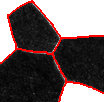
\includegraphics[width=0.32\linewidth]{fig/aac}}
\caption{Example selection of a spurious segment $S^V_k$ for removal.
  \textbf{(a)} Chosen $S^V_k$ and surrounding segments.  \textbf{(b)}
  Local region extracted around $S^V_k$.  \textbf{(c)} The updated
  segmentation in the extracted local region.}
\label{fig:removal-ex}
\end{figure}

For ease of notation, we use similar notation to the adjacency
definition in \eq{phi} by using $\{\mathcal{A}^V\}_k$ to refer to the
set of segments neighboring the segment $S^V_k$.  This way, the local
region for updating the segmentation is
\begin{equation}
  \mathcal{L} = \{\mathcal{A}^V\}_k \bigcup S^V_k .
\end{equation}

In this local region, we rerun the energy minimization of \eq{energy1}
by modifying the $\Theta$ term.  In particular, we do not allow any
pixel to be assigned to $S^V_k$ since this segment is to be removed.
Instead, the pixels initially in $S^V_k$ can be assigned to any of the
segments in $\{\mathcal{A}^V\}_k$ with $0$ cost for the $\Theta$ term,
\ie,
\begin{equation}\label{eq:remove}
\begin{aligned}
 \forall p \in S^V_k ,& \quad \Theta_p(\tilde{S}^V_i) = \left\{
   \begin{array}{lcr}
     0, & S^V_i \in \{\mathcal{A}^V\}_k  \\
     \infty, & \textrm{ otherwise} \\
   \end{array}
 \right. \\
\forall p \notin S^V_k ,& \quad \Theta_p(\tilde{S}^V_i) = \Theta_p(S^V_i)
\end{aligned}
\end{equation}
By updating $\Theta$ in this fashion, we do not require the pixels
previously in $S^V_k$ merged into a single neighboring segment.
Instead, these pixels may be assigned to more than one segment in
$\{\mathcal{A}^V\}_k$, as shown in \figsub{removal-ex}{b}.

Note that this interaction is very simple and convenient, as it
requires only a single click anywhere inside the spurious segment
$S^V_k$.  The full algorithm for removing spurious segments is
summarized in \alg{remove}.
\begin{algorithm}[!t]
  \centering
  \algrenewcommand\algorithmicforall{\textbf{for each}}
  \begin{algorithmic}[1]
    \Function{RemoveSegment}{$S^V, S^V_k$}
    % \State $A_k \gets$ neighbors for $S^V_k$
    \State $\mathcal{L} \gets \{\mathcal{A}^V\}_k \bigcup S^V_k$
    \State $\forall p \in \mathcal{L}$, build graph for energy minimization problem from~\cite{waggoner:11}
    \State $\Theta \gets $ set from \eq{remove}
    \State $\tilde{S}^V \gets S^V$ incorporating the updated segmentation in $\mathcal{L}$
    \State \textbf{return} updated $\tilde{S}^V$
    \EndFunction
  \end{algorithmic}
  \caption{Interactively specifying segment to remove.}
  \label{alg:remove}
\end{algorithm}

\subsection{Addition of Missing Segments}
\label{sec:addition}

Unlike removal, interactively annotating an additional structure
cannot be solely formulated as a simple modification of the $\Theta$
term in the energy minimization formulation.  This is because the
multi-labeling problem used to optimize the energy minimization form
in \eq{energy1} optimizes over a fixed set of segments, and cannot
introduce new segments.  Thus, for each missing segment, we must
explicitly create a new segment at the location interactively
specified by the user.

Based on the initial segmentation $S^V = \{ S^V_1, S^V_2, \ldots,
S^V_n \} $, we take as input from the user an annotation specifying
the center location $c$ of the new segment $\tilde{S}^V_{n+1}$.  In
addition to this, we also accept two parameters from the user: 1) the
\emph{seed} radius $s$ specifying a circular region around $c$ such
that this circular region is completely contained within the missing
structure; 2) a \textit{dilation} radius $d$, which is similar to the
dilation parameter used in~\cite{waggoner:11}, such that the circular
region with this dilation radius $d$ centered at $c$ completely covers
the missing structure to be segmented.  We explicitly enforce that $d
\geq s$ for any choice of $s$.  We call pixels within the seed radius
$s$ of $c$ ``seed pixels'' and pixels within the dilation radius $d$
of $c$ ``dilation pixels.''  In this interaction, seed pixels are
\emph{guaranteed} to be part of the missing segment that is added, as
shown by the green circle in \figsub{addition-ex}{b}, and dilation
pixels, excluding seed pixels, are \emph{potentially} part of the
missing segment that is added, as shown by the blue area in
\figsub{addition-ex}{b}.  This makes the selection of $s$ and $d$
conceptually simple for the user to tune.  In \sect{param}, we discuss
how to automate the selection of $s$ and $d$ to further reduce the
user's burden when interactively segmenting a materials volume.
\begin{figure}[htbp]
\centering
\subfloat[]{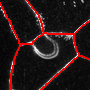
\includegraphics[width=0.30\linewidth]{fig/bba}}
\hspace{0.1em}
\subfloat[]{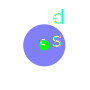
\includegraphics[width=0.30\linewidth]{fig/bbb.pdf}}
\hspace{0.1em}
\subfloat[]{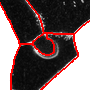
\includegraphics[width=0.30\linewidth]{fig/bbd}}
\caption{Annotating the addition of a missing segment.  \textbf{(a)}
  Segmentation $S^V$ with a missing segment near the center of the
  image.  \textbf{(b)} Annotation of a center point $c$, along with a
  seed radius $s$ and a dilation radius $d$, and the identified local
  region for updating the segmentation.  \textbf{(c)} The updated
  segmentation of the local region shown in (b).} 
\label{fig:addition-ex}
\end{figure}

Similar to the removal interaction in \sect{remove}, we define a local
region around the specified $c$ to update the segmentation of $S^V$.
Specifically, we define this region by taking all segments in $S^V$
that contain one or more seed or dilation pixels.  In this local
region we modify the $\Theta$ term of the energy minimization in
\eq{energy1} to obtain an updated segmentation.  Specifically, we
allow all seed and dilation pixels to be reassigned to the new segment
$\tilde{S}^V_{n+1}$ by setting
\begin{equation}
  \label{eq:d}
  \Theta_p(\tilde{S}^V_{n+1}) = \left\{
    \begin{array}{lcr}
      0, & \| p - c \| \leq d  \\
      \infty, & \textrm{ otherwise} \\
    \end{array}
  \right.
\end{equation}
where $\| \cdot \|$ is the euclidean distance between pixels $p$ and
$c$.  %% Though this is necessary to include the new segment in the
%% energy minimization, it is not sufficient to guarantee that it will
%% appear in the final segmentation.
Furthermore, to insure that the seed pixels are always guaranteed to
be part of $\tilde{S}^V_{n+1}$ we set an infinity penalty for seed
pixels assigned to any segment other than $\tilde{S}^V_{n+1}$, 
\begin{equation}
  \label{eq:s}
  \Theta_p(\tilde{S}^V_i) = \left\{
    \begin{array}{lcr}
      \infty, & \| p - c \| \leq s \textrm{ and } i \neq n+1  \\
      \Theta_p(S^{V}_i), & \textrm{ otherwise.} \\
    \end{array}
  \right.
\end{equation}
The full algorithm for adding a missing segment is summarized in
\alg{addition}.
\begin{algorithm}[!t]
  \centering
  \algrenewcommand\algorithmicforall{\textbf{for each}}
  \begin{algorithmic}[1]
    \Function{AddSegment}{$S^V, c$, $s$, $d$}
    \State $\mathcal{L} \gets$ union of all segments that contain a seed pixel or dilation pixel
    \State $\forall p \in \mathcal{L}$, build graph for energy minimization problem from~\cite{waggoner:11}
    \State $\Theta \gets $ set from \eq{d} and \eq{s}
    %% \State $\tilde{S}^V \gets S^V$ updated with the pixels assigned in $\mathcal{L}$
    \State $\tilde{S}^V \gets S^V$ incorporating the updated segmentation in $\mathcal{L}$
    % \State $ \tilde{S}^V \gets $ minimization of energy in local region and copied to $S^V$
    \State \textbf{return} updated $\tilde{S}^V$
    \EndFunction
  \end{algorithmic}
  \caption{Interactively specifying segment to add.}
  \label{alg:addition}
\end{algorithm}

\section{Parameter Estimation}
\label{sec:param}

When interactively adding a new segment, as discussed in
\sect{addition}, the seed radius $s$ and dilation radius $d$ are
required to be specified by the user.  This results in additional
burden on the part of the user.  In this section, we develop a
parameter estimation approach to automatically select these two
parameters so the user need only override them in very rare cases, or
not at all.

We do this by leveraging information about the center $c$ the user
provided relative to the initial segment in which it resides.
Generally a missing segment occurs when 2D cross-section intersects a
new 3D structure in $V$.  Given a small inter-slice distance, we
expect that these missing segments are often small compared with its
neighboring segments in slice $V$.  An example is shown in
\figsub{param}{a}, where a small segment is missing (indicated by the
yellow circle) in the segmentation $S^V$: this missing segment is
mistakenly merged into a large neighboring segment $S^V_b$.
Intuitively, placing $c$ near the boundary of $S^V_b$ likely indicates
the missing segment is small, as shown by \figsub{param}{b}.
Conversely, placing $c$ closer to the center of $S^V_b$ likely
indicates the resulting missing segment is large as shown in
\figsub{param}{c}.  We make a simplifying assumption that we do not
allow the missing segment to spill over the boundary of $S^V_b$.  For
example, the selection of $c$ and $s$ in \figsub{param}{b} is able to
generate the updated segmentation shown in \figsub{param}{d}.
\begin{figure}[htbp]
\centering
\subfloat[]{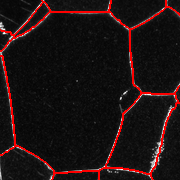
\includegraphics[width=0.30\linewidth]{fig/cca.pdf}}
\hspace{0.1em}
\subfloat[]{
\includegraphics[width=0.30\linewidth]{fig/ccf.pdf}}

\subfloat[]{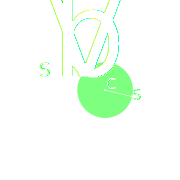
\includegraphics[width=0.30\linewidth]{fig/ccg.pdf}}
\hspace{0.1em}
\subfloat[]{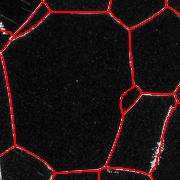
\includegraphics[width=0.30\linewidth]{fig/ccb.pdf}}
\caption{Automatic selection of seed radius~$s$ and dilation
  radius~$d$.  \textbf{(a)}~A missing segment located within a large
  segment in $S^V_b$.  \textbf{(b-c)}~Selections of~$c$ at varying
  distances from the boundary of $S^V_b$, resulting in different
  estimations of~$s$.  \textbf{(d)}~Updated $\tilde{S}^V$ by adding
  a missing segment using the $c$ shown~(b) and the proposed parameter
  estimation method to determine $s$.} \label{fig:param}
\end{figure}

To obtain an estimation of $s$ we start by setting $s=0$, and we then
increase $s$ by a small $\epsilon$ amount until the circle centered at
$c$ with radius $s$ is within $\epsilon$ distance of the boundary of
the containing segment $S^V_b$, as shown by the arrow in
\figsub{ex}{b-c}.  In materials images, the majority of
newly-appearing structures when moving from one slice to another are
usually near the boundary of an existing structure $S^V_b$ (near a
``Y''-junction boundary between structures).  This automatic approach
is ideally suited for these cases.  When the user specifies a $c$ that
falls directly on a segment boundary in $S^V$, we default to requiring
user-supplied $s$ in these less-common cases.  For estimating $d$, it
is scaled according to the value of $s$.  Specifically, we set $d =
2\cdot s$.  As shown in \sect{ex}, this approach saves both time and
effort.

%% Similar to this, we obtain
%% an estimation of $d$ by starting it at the estimated size of $s$, and
%% then incrementally increase it by $\epsilon$.  There is not a simple
%% stopping criterion to know undoubtedly that $d$ covers the entire
%% substructure desired.  However, we observe that if we separate the
%% containing segment into a background, and everything outside of the
%% containing segment into foreground, and we stop increasing $d$ when it
%% encompasses two, connected foreground regions, we tend to obtain a
%% large-enough value for $d$.  If this stopping condition never occurs,
%% we enforce a fixed maximum for $d$.  An illustration is given in
%% \fig{d-size}, where the $d$ size (blue circle) is not large enough in
%% \figsub{d-size}{a} and contains only a single connected foreground
%% component, whereas in \figsub{d-size}{b}, the $d$ size contains two
%% disjoint foreground regions, thus meeting the stopping criteria.
%% \begin{figure}[htbp]
%% \centering
%% \subfloat[Single foreground component]{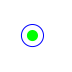
\includegraphics[width=0.30\linewidth]{fig/cce}}
%% \hspace{0.1em}
%% \subfloat[Two foreground components]{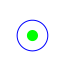
\includegraphics[width=0.30\linewidth]{fig/ccd.pdf}}
%% \caption{} \label{fig:d-size}
%% \end{figure}

\section{Experiments}
\label{sec:ex}

To evaluate the proposed interactive segmentation method, we use it to
segment a sequence of~$11$ (indexed from $0$ to $10$) microscopic
titanium images~\cite{rowenhorst:10} provided by Dave Rowenhorst, NRL.
We measure the effort (\ie, number of clicks) used to segment each
slice in the dataset, as well as the overall time expended by the user
to segment a slice.  The previous segmentation propagation
approach~\cite{waggoner:11} requires a complete segmentation on one
slice as an initialization.  We count the manual segmentation on this
initial slice into the effort and time required.  We present the
proposed method both with and without using the automatic parameter
estimation discussed in \sect{param}.

For comparison, we use the readily-available ``intelligent scissors''
interactive segmentation method~\cite{mortensen:95}.  Using the
intelligent scissors tool, we independently segment all $11$ slices
from the same dataset, evaluating both effort (number of clicks) and
time.  In addition, we produce a hybrid of our previous automatic
method~\cite{waggoner:11} and the intelligent scissors method, which
we call ``intelligent scissors + propagation'' in \fig{ex}.  This
approach uses the method from~\cite{waggoner:11} to propagate a
segmentation from an initial slice to the remaining slices, but it
uses the intelligent scissors tool~\cite{mortensen:95} to carry out
the interactive component instead of the interaction proposed in this
paper.

The results of this comparative experiment are shown in \fig{ex}.
Note that, in propagated methods (``Proposed,'' ``Proposed + Parameter
Estimation,'' and ``Intelligent Scissors + Propagation''), the first
slice is used as the initial slice $U$, so it requires significantly
more effort and time to segment compared with the remaining slices.
\begin{figure}[htbp]
\centering
\subfloat[Effort]{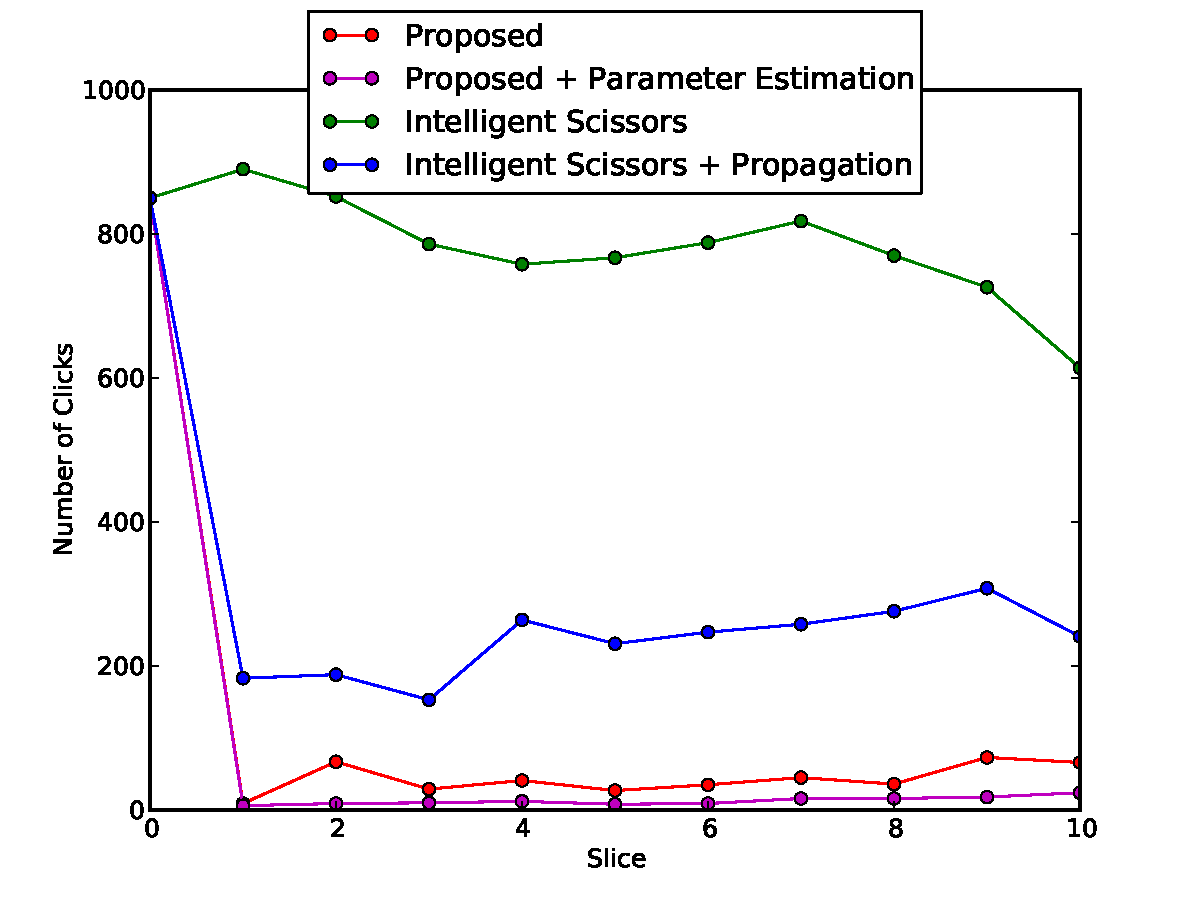
\includegraphics[width=0.48\linewidth]{fig/eval}}
\hspace{0.1em}
\subfloat[Time]{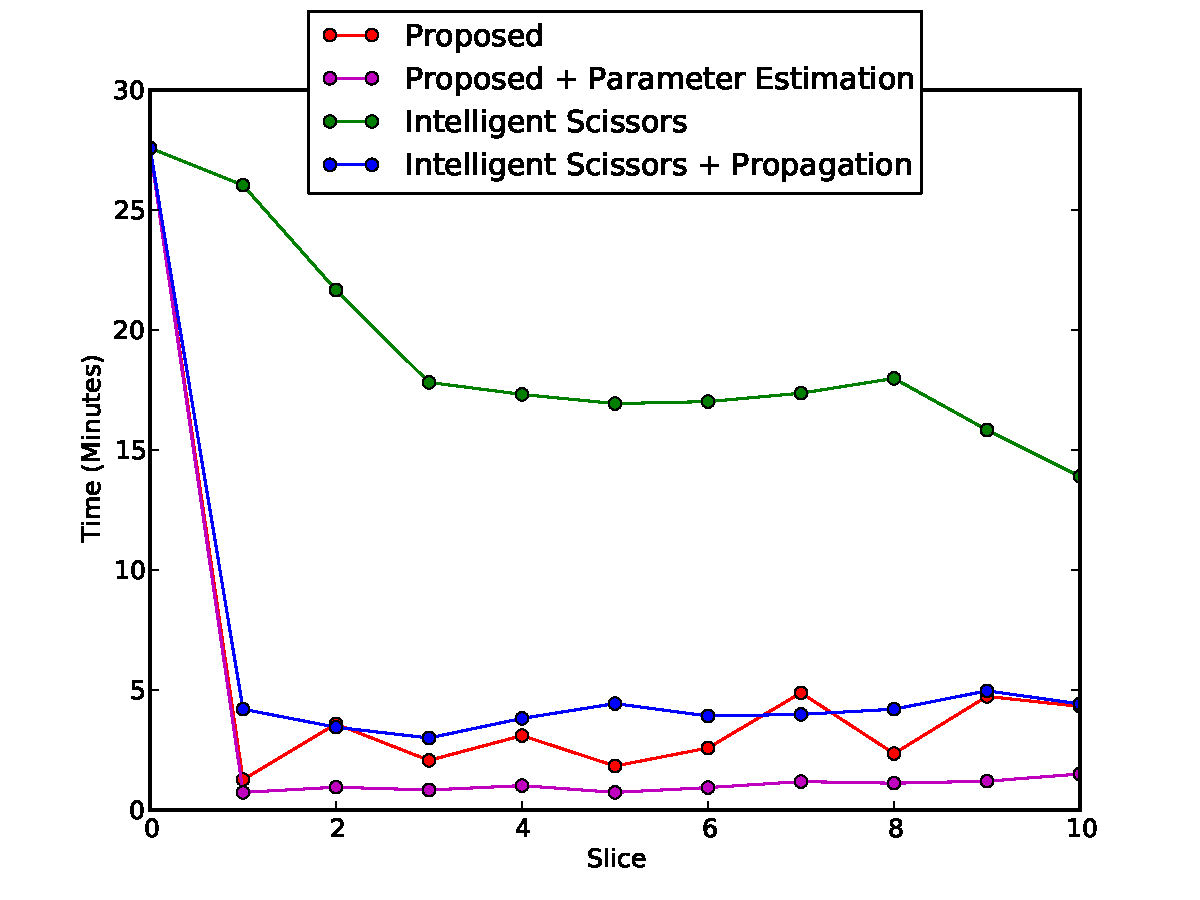
\includegraphics[width=0.48\linewidth]{fig/eval_time}}
\caption{Evaluation of \textbf{(a)} the amount of effort (number of
  clicks) and \textbf{(b)} time taken for a user to interactively
  segment the 11 sample slices.  Smaller values are better, for both
  figures.} \label{fig:ex}
\end{figure}
From \fig{ex}, we can see that the method proposed in this paper
(``Proposed'') allows much more rapid segmentation time ($< 5$ minutes
in most cases) and with much less effort ($< 100$ clicks in most
cases) compared with the unpropagated intelligent scissors method.
The intelligent scissors method (``Intelligent Scissors''), without
the benefit of propagation, requires significantly more time and
effort.  The hybrid method (``Intelligent Scissors + Propagation'')
fares better than the unpropagated intelligent scissors method, but it
still requires greater effort than the proposed method.  Finally, the
proposed parameter estimation method (``Proposed + Parameter
Estimation'') can further reduce both the time and effort required by
the proposed method.

\begin{figure}[htbp]
\centering
\subfloat[F-measure]{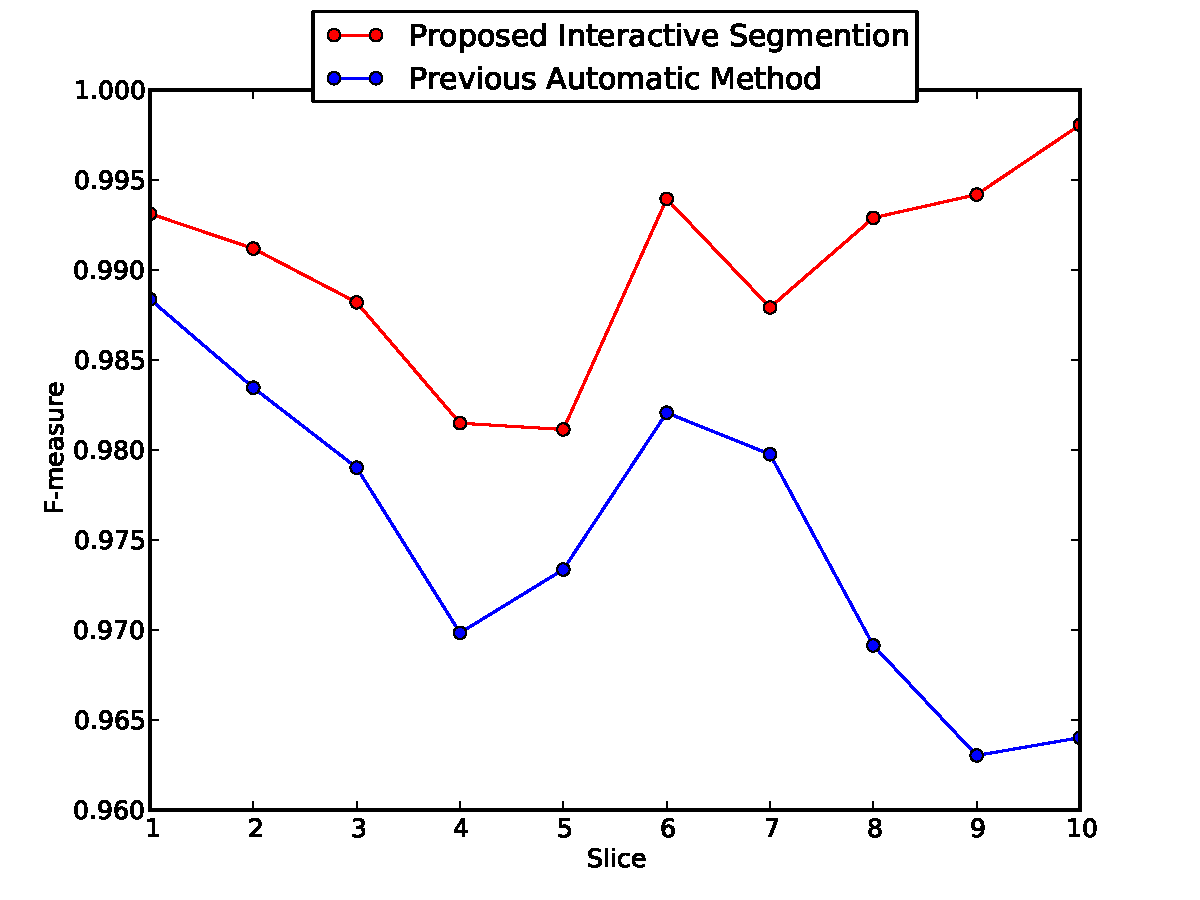
\includegraphics[width=0.44\linewidth]{fig/eval_f}}

\subfloat[Precision]{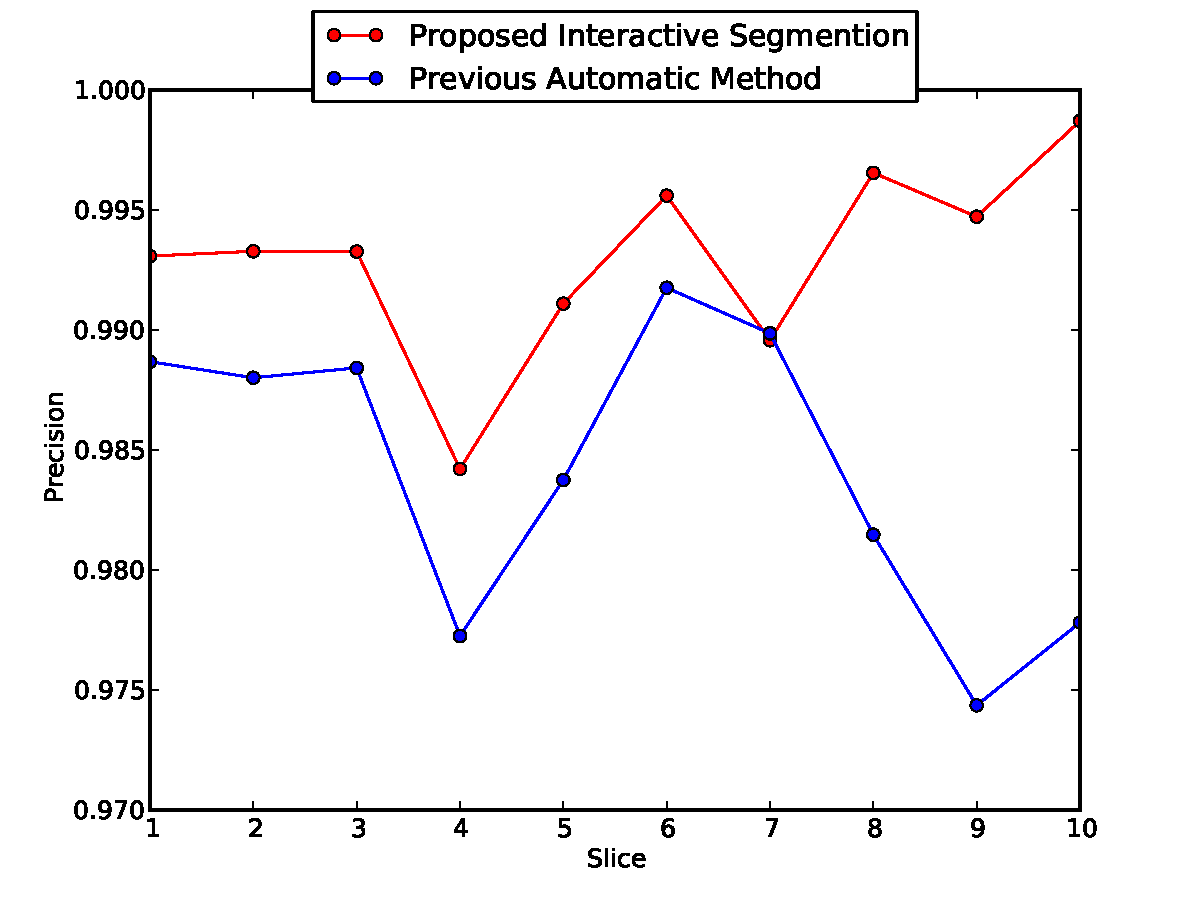
\includegraphics[width=0.4\linewidth]{fig/eval_p}}
\hspace{0.1em}
\subfloat[Recall]{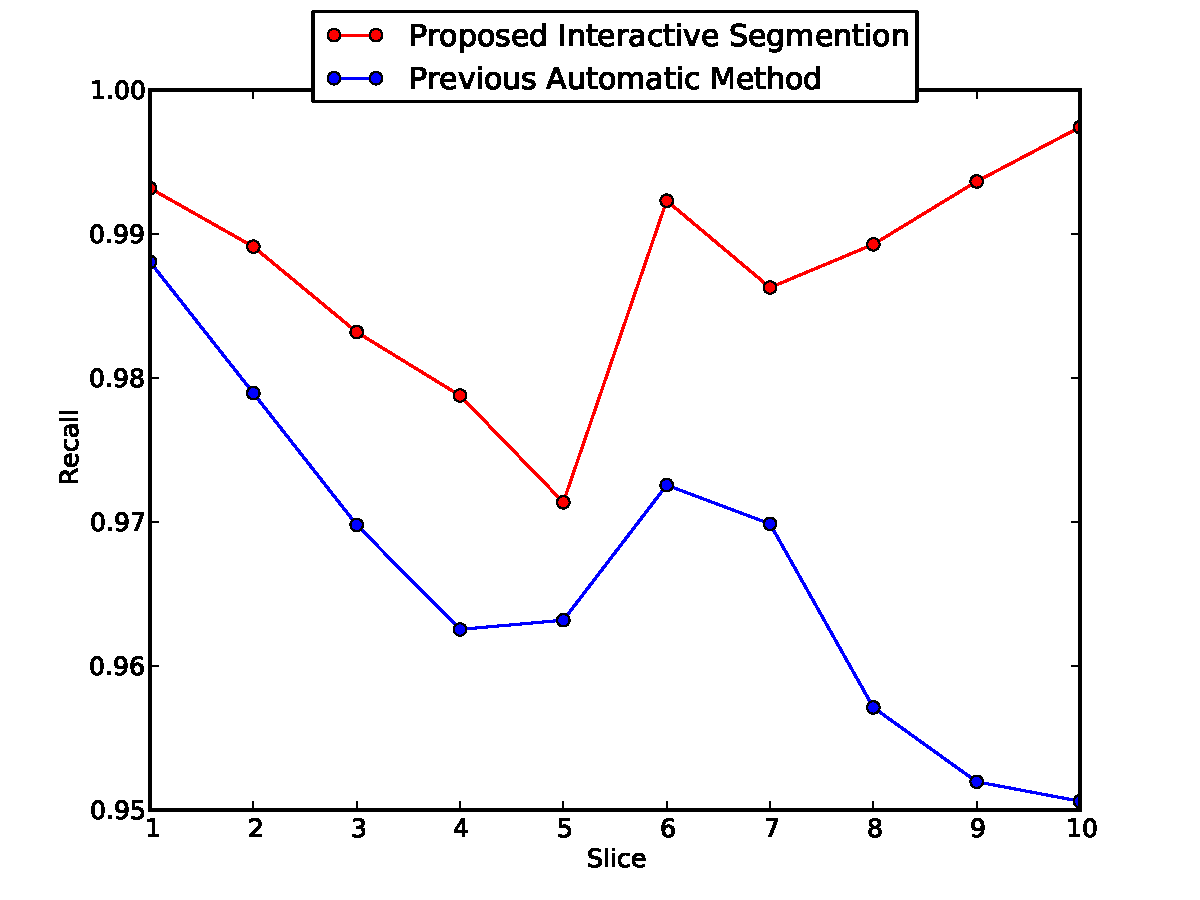
\includegraphics[width=0.4\linewidth]{fig/eval_r}}
\caption{Performance of the proposed interactive segmentation method
  compared with our previous automated method~\cite{waggoner:11}
  measured by the boundary coincidence with the ground truth
  segmentation.}
\label{fig:perform}
\end{figure}

In \fig{perform}, we show that the proposed interactive method is able
to increase the segmentation accuracy of our state-of-the-art
materials image segmentation method in~\cite{waggoner:11}.  As in our
previous work~\cite{waggoner:11}, we use the precision, recall, and
F-measure, which is the harmonic mean of the precision and
recall~\cite{martin:01}, to show the segment boundary coincidence with
the manually-constructed ground truth segmentation.  For both the
proposed and previous automatic methods, we propagate from an initial
slice $0$ to the remaining $10$ slices, and the proposed
interaction-enhanced method increases performance for all slices.
Finally, qualitative segmentation results using the proposed
interactive method are shown in \fig{qual} where we show the automatic
segmentation results with spurious or missing segments, the human
annotation, and the updated segmentation.

\begin{figure}[htbp]
%% \renewcommand{\thesubfigure}{\thefigure.\arabic{subfigure}}
\setlength{\tabcolsep}{0.2em}

\centering

\subfloat[]{\begin{tabular}{ccc} 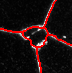
\includegraphics[width=0.15\linewidth]{fig/qual/a1} &
    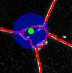
\includegraphics[width=0.15\linewidth]{fig/qual/a2} &
    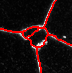
\includegraphics[width=0.15\linewidth]{fig/qual/a3} \end{tabular}} \hspace{1em}
\subfloat[]{\begin{tabular}{ccc} 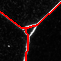
\includegraphics[width=0.15\linewidth]{fig/qual/b1} &
    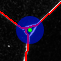
\includegraphics[width=0.15\linewidth]{fig/qual/b2} &
    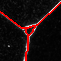
\includegraphics[width=0.15\linewidth]{fig/qual/b3} \end{tabular}}

\subfloat[]{\begin{tabular}{ccc} 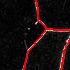
\includegraphics[width=0.15\linewidth]{fig/qual/c1} &
    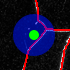
\includegraphics[width=0.15\linewidth]{fig/qual/c2} &
    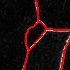
\includegraphics[width=0.15\linewidth]{fig/qual/c3} \end{tabular}} \hspace{1em}
\subfloat[]{\begin{tabular}{ccc} 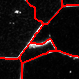
\includegraphics[width=0.15\linewidth]{fig/qual/d1} &
    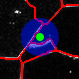
\includegraphics[width=0.15\linewidth]{fig/qual/d2} &
    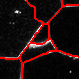
\includegraphics[width=0.15\linewidth]{fig/qual/d3} \end{tabular}}

\subfloat[]{\begin{tabular}{ccc} 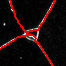
\includegraphics[width=0.15\linewidth]{fig/qual/e1} &
    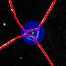
\includegraphics[width=0.15\linewidth]{fig/qual/e2} &
    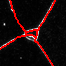
\includegraphics[width=0.15\linewidth]{fig/qual/e3} \end{tabular}} \hspace{1em}
\subfloat[]{\begin{tabular}{ccc} 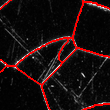
\includegraphics[width=0.15\linewidth]{fig/qual/f1} &
    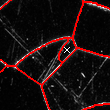
\includegraphics[width=0.15\linewidth]{fig/qual/f2} &
    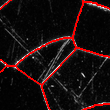
\includegraphics[width=0.15\linewidth]{fig/qual/f3} \end{tabular}}

\subfloat[]{\begin{tabular}{ccc} 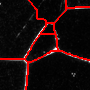
\includegraphics[width=0.15\linewidth]{fig/qual/g1} &
    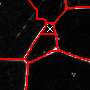
\includegraphics[width=0.15\linewidth]{fig/qual/g2} &
    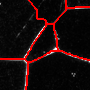
\includegraphics[width=0.15\linewidth]{fig/qual/g3} \end{tabular}} \hspace{1em}
\subfloat[]{\begin{tabular}{ccc} 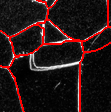
\includegraphics[width=0.15\linewidth]{fig/qual/h1} &
    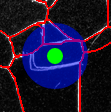
\includegraphics[width=0.15\linewidth]{fig/qual/h2} &
    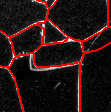
\includegraphics[width=0.15\linewidth]{fig/qual/h3} \end{tabular}}

\subfloat[]{\begin{tabular}{ccc} 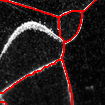
\includegraphics[width=0.15\linewidth]{fig/qual/i1} &
    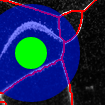
\includegraphics[width=0.15\linewidth]{fig/qual/i2} &
    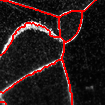
\includegraphics[width=0.15\linewidth]{fig/qual/i3} \end{tabular}} \hspace{1em}
\subfloat[]{\begin{tabular}{ccc} 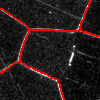
\includegraphics[width=0.15\linewidth]{fig/qual/j1} &
    \includegraphics[width=0.15\linewidth]{fig/qual/j2} &
    \includegraphics[width=0.15\linewidth]{fig/qual/j3} \end{tabular}}

\caption{Qualitative results where each subfigure shows the initial
  automatic segmentation $S^V$ (left); the human annotation (middle)
  with the seed pixels in green and dilation pixels in blue, and
  ``X''s indicating spurious segments to be removed; and the updated
  segmentation $\tilde{S}^V$ (right).  Note that (f) and (g)
  illustrate removal annotation and the remaining illustrate addition
  annotation.}
\label{fig:qual}
\end{figure}

\section{Conclusion}
\label{sec:conclusion}

We have presented an interactive segmentation method extended from our
automatic segmentation propagation approach.  By allowing the user to
interactively handle spurious and missing segments when propagating
from one slice to another, we show that the time required to segment a
materials image volume, as well as the overall effort (number of
clicks) needed for interaction, is much less than the comparison
``intelligent scissors'' method used in popular image processing
tools.  By updating the segmentation within a local region around the
interactive annotation, we are able to obtain a fast, yet robust means
to handle segmentation errors when a new structure appears or an
existing structure disappears from the 2D cross-section of a
particular slice of the volume.  We also introduce a simple automatic
technique to estimate the seed radius when adding a missing segment.
We show that this can further reduce the amount of time and effort
needed by the proposed approach.

\bibliography{matsci}
\bibliographystyle{spiebib}   %>>>> makes bibtex use spiebib.bst

\end{document} 
